\newcommand{\TITLE}{Algorithms Lab}
\newcommand{\SUBTITLE}{The comprehensive guide}

\theoremstyle{plain}
\newtheorem{thm}{Theorem}[section]
\theoremstyle{definition}
\newmdtheoremenv{mistake}[thm]{Mistake}

% \nointent everywhere
\setlength\parindent{0pt}

\newenvironment{mt}[1]{
  \begin{mistake}
    #1\\

}{
\end{mistake}
}

\newenvironment{fx}{
  \textbf{Fix.} 
}{
}

\usepackage{minted}
\newcommand{\cl}[1]{\mintinline{raw}{#1}}
\newcommand{\cc}[1]{\mintinline{c++}{#1}}

\newcommand{\examplell}[3]{
  \begin{figure}[H]
    \centering
    \begin{mdframed}
      \inputminted[firstline=#2, lastline=#3]{c++}{examples/#1.cc}
    \end{mdframed}
  \end{figure}
}

\newcommand{\example}[1]{
  \begin{figure}[H]
    \centering
    \begin{mdframed}
      \inputminted{c++}{examples/#1.cc}
    \end{mdframed}
  \end{figure}
}

\newmdtheoremenv{mathtip}[thm]{Math Tip}
\newenvironment{matht}[1]{
  \begin{mathtip}
    #1
    \newline
}{
\end{mathtip}
}

% Fancy headers and footers
\usepackage{fancyhdr}
\pagestyle{fancy}
\lhead{Algorithms Lab Solutions}
\rhead{\thepage}
\cfoot{Tom Sydney Kerckhove}
\renewcommand{\headrulewidth}{0.4pt}
\renewcommand{\footrulewidth}{0.4pt}


\newcommand{\includesolution}[1]{
  \def\curdir{../src/#1}
  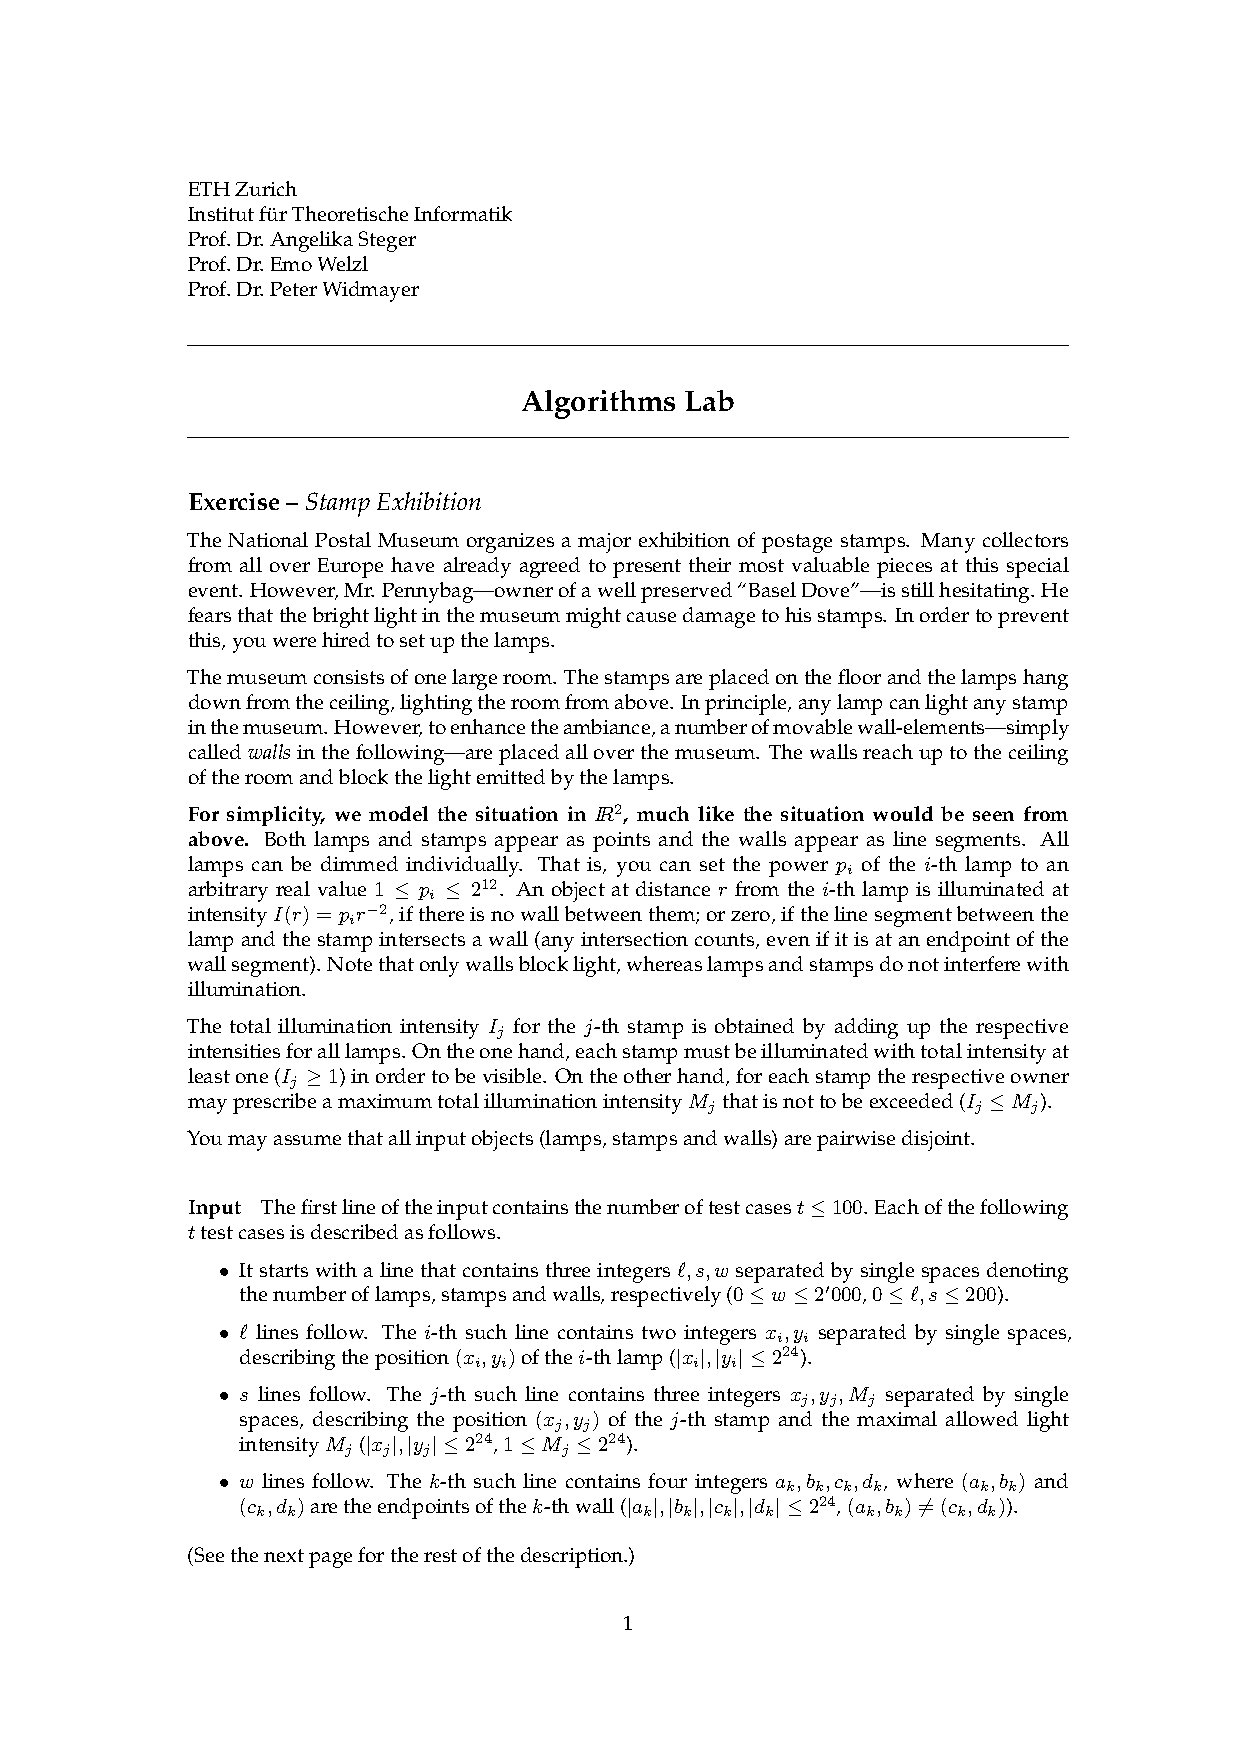
\includepdf[pages=-]{\curdir/assignment.pdf}
  \subfile{\curdir/writeup}
  \newpage\inputminted[fontsize=\scriptsize]{c++}{\curdir/main.cc}
}


% Inputting code
\newcommand\code[3]{
  \begin{figure}[H]
    \centering
    \begin{mdframed}
      \inputminted[firstline=#2, lastline=#3]{c++}{\currfileabsdir#1.cc}
    \end{mdframed}
  \end{figure}
}

% Styles
\newenvironment{solutions}
{}
{}
\newenvironment{solution}[3]
{
  \section{#1}
  \subsection*{Time: $O\left(#2\right)$, Space: $O\left(#3\right)$}
}
{}

% For tags
\newcommand{\bx}[1]{ \framebox[1.1\width]{#1} }
\newcommand{\tagged}[1]{\bx{#1}}


